\chapter{Soporte del Robot LEGO Ev3 Físico}
\chaptermark{Soporte Físico}
Ahora nos centraremos en cuál ha sido el desarrollo seguido para que el bloque \textit{Ev3} reciba código desde un cliente exterior y pueda ejecutarlo en local. Primero, el \textit{driver} en \textit{Python} que permite a las aplicaciones de los usuarios de \textit{Kibotics} recibir las lecturas de los sensores del robot real u ordenar movimiento a sus motores. Y luego cómo integrarlo de modo que el programa se descargue en el robot real desde la página web de \textit{Kibotics}

\section{Interfaz de programación de sensores y actuadores}
\sectionmark{Interfaz de programación}
\label{sec:interfazfisico}
Para crear los \textit{drivers} de \textit{Kibotics} del robot \textit{LEGO EV3} real se ha utilizado la librería \texttt{ev3dev2} donde se encuentran las funciones necesarias para el control del robot en Python 

\subsection{Soporte de actuadores}
Los motores son los actuadores y la forma de uso de \textit{Kibotics} es la de \textit{Tracción diferencial}, en el cual los motores se mueven a la par. Por lo tanto para crear las funciones  del \textit{HAL API} en Python voy a utilizar la clase \textit{MoveTank} dentro de la librería de \texttt{ev3dev2} \footnote{\url{https://github.com/ev3dev/ev3dev-lang-python}} .
 
\begin{lstlisting}[frame=single,breaklines=true, label=Clase MoveTank caption=Clase MoveTank,  captionpos=b]

class MoveTank(MotorSet):
    """
    Controls a pair of motors simultaneously, via individual speed setpoints for each motor.

    Example:

    .. code:: python

        tank_drive = MoveTank(OUTPUT_A, OUTPUT_B)
        # drive in a turn for 10 rotations of the outer motor
        tank_drive.on_for_rotations(50, 75, 10)
    """
    def __init__(self, left_motor_port, right_motor_port, desc=None, motor_class=LargeMotor):
        motor_specs = {
            left_motor_port: motor_class,
            right_motor_port: motor_class,
        }

        MotorSet.__init__(self, motor_specs, desc)
        self.left_motor = self.motors[left_motor_port]
        self.right_motor = self.motors[right_motor_port]
        self.max_speed = self.left_motor.max_speed
        self._cs = None
        self._gyro = None
\end{lstlisting}

En esta clase se encuentran todos los métodos con los que construiré mi \textit{Driver}


\begin{lstlisting}[frame=single,breaklines=true, label=Driver Actuadores, caption=Drivers,  captionpos=b]


import ev3dev2.motor
import time


class Ev3Wrapper:

    def __init__(self,
                 left_motor_port=OUTPUT_D,
                 right_motor_port=OUTPUT_A):


        tank_drive = MoveTank(left_motor_port, right_motor_port)


    def TurnDegrees(self, degrees, speed):
        # get the starting position of each motor
        tank_drive.turn_degrees(self, speed, degrees)

    def avanzar(self, val):
        tank_drive.on(self,val, val)

    def retroceder(self, val):
        tank_drive.on(self,-val,-val)

    def girar_derecha(self, w):

        tank_drive.turn_right(self, 360, 2*3,1416/w)

    def girar_izquierda(self, w):

        tank_drive.turn_left(self, 360, 2*3,1416/w)

    def avanzar_hasta(self, distance):
        dist_mm = distance * 1000

        # the number of degrees each wheel needs to turn
        tank_drive.on_for_distance(self, 20, distance_mm, brake=True, block=True)

    def retroceder_hasta(self, distance):
        self.avanzar_hasta(-distance)

    def girar_derecha_hasta(self, degrees):
        self.TurnDegrees(degrees, 20)

    def girar_izquierda_hasta(self, degrees):
        self.TurnDegrees(-degrees, 20)

    def parar(self):
        tank_drive.odometry_stop()


    def target_reached(self,left_target_degrees,right_target_degrees):
        tolerance = 5
        min_left_target = left_target_degrees - tolerance
        max_left_target = left_target_degrees + tolerance
        min_right_target = right_target_degrees - tolerance
        max_right_target = right_target_degrees + tolerance

        current_left_position = left_motor_port.position()
        current_right_position = right_motor_port.position()

        if current_left_position > min_left_target and \
           current_left_position < max_left_target and \
           current_right_position > min_right_target and \
           current_right_position < max_right_target:
            return True
        else:
            return False
\end{lstlisting}


\subsection{Soporte de sensores}
Dentro de los sensores soportados por el \textit{HAL API} de \textit{Kibotics} hay algunos que no se pueden aplicar al robot \textit{LEGO EV3} ya que no dispone de sensores, como la cámara o el sensor de Infrarrojos. Por lo que los \textit{drivers} que se incluirán en este apartado son:

\begin{table}[H]
\caption{Métodos (HAL API) soportados por Ev3.}
\vspace{0.5cm}
\label{tab:tablaSensores}
\resizebox{\textwidth}{!}{%
\begin{tabular}{|c|c|c|ll}
\cline{1-3}
\textbf{Método} & \textbf{Descripción} & \textbf{Salida} &  &  \\ \cline{1-3}
.getDistance() & \begin{tabular}[c]{@{}c@{}}Devuelve la distancia entre el robot\\  y la intersección del raycaster en el centro\end{tabular} & number(metros) &  &  \\ \cline{1-3}
.IsTouching() & Devuelve si algo presiona el sensor & Boolean &  &  \\ \cline{1-3}
.getObjectColor(color) & \begin{tabular}[c]{@{}c@{}}Devuelve un objeto con la posición del elemento\\ detectado por la cámara del color pasado por parámetro\end{tabular} & \begin{tabular}[c]{@{}c@{}}\{center:{[}x.y{]},\\ area: int\}\end{tabular} &  &  \\ \cline{1-3}



\end{tabular}%
}
\end{table}

Para este \textit{driver} utilizaré las funciones definidas en el API de \texttt{Ev3dev2.sensor}, las cuales incluyen todas los sensores que puede llevar el \textit{LEGO EV3}. Pero solo utilizaremos las clases \texttt{TouchSensor(), ColorSensor() y Ultrasonic()} que son los tres sensores que usamos en este proyecto. 

\begin{lstlisting}[frame=single,breaklines=true, label=Driver Actuadores, caption=Drivers,  captionpos=b]
from ev3dev2.sensor import INPUT_1, INPUT_2, INPUT_3, INPUT_4
import ev3dev2.sensor.lego
import time


class Ev3Wrapper:

    def __init__(self):
        us= UltraSonic()
        to= TouchSensor()
        cs = ColorSensor()


    def getObjectColor(self, color):
        cs.color()

    def getDistance(self):
        us.distance_centimeters_continuous()

    def isTouching(self):
        to.is_pressed()
\end{lstlisting}

\section{Descarga desde la plataforma}

En la figura se muestra el diseño seguido para integrar el Ev3 real a la plataforma Kibotics. El proceso consta de 4 pasos y en las siguientes secciones se profundizará en cada una de las partes y en las interacciones necesarias entre el cliente, el servidor de Kibotics y el servidor \textit{Flask} que lanzaremos en el \textit{Robot Ev3},lo que permitira programarlo desde el navegador web usando  \textit{Kibotics}.

\begin{figure}[h!]
  \centering
    \includegraphics[width=0.8\textwidth]{img/esquema.JPG}
  \caption{Diseño para la integración del Ev3}
  \label{comunicacion}
\end{figure}

\subsection{Preparación ordenador a bordo del robot}
Lo primero para la recepción de mensajes es tener un dispositivo que pueda recibirlos, en este caso tendremos que instalar en el \textit{LEGO EV3} un sistema operativo que permita desplegar un servidor. Comenzaré hablando del apartado técnico del robot, para entender la solución adoptada. El Bloque \textit{Ev3} es la mejora de su predecesor el \textit{LEGO NXT}, añadiéndole mas potencia, memoria y expandibilidad. Cuenta con un procesador ARM9 a 300 MHz con memoria Flash de 16 MB, 64 MB de RAM y memoria ampliable con tarjetas mini SD hasta 32 GB. Ademas de eso dispone de conexiones \textit{Bluetoooth 2.1} y puerto USB. 

\begin{wrapfigure}{l}{0.3\linewidth}
    \centering
    
\includegraphics[width=0.6\linewidth]{img/logo_ev3dev_mono.png}
    \caption{Ev3Dev Logo}
    \label{fig:ev3dev}
\end{wrapfigure}

\textit{Ev3Dev}\footnote{\url{https://www.ev3dev.org/}} es un sistema operativo basado en \textit{Debian-Linux} diseñadoespecialmente para el \textit{LEGO MINDSTORM EV3} , haciendo ingeniería inversa del bloque.\newline
Una vez instalada la imagen en el robot, para tener conexión a Internet hay dos opciones. La más simple es conectar un \textit{Wifi Dongle} al puerto USB del Bloque \textit{Ev3}, y se accede a la red \textit{Wifi} como cualquier ordenador. La segunda opción es conectar por cable el robot a tu ordenador, y conectarlo a la red como una extensión de tu red.\newline
Una vez conectado a Internet, ya puedes conectarte al robot vía \textit{SSH}.

\begin{figure}[h!]
  \centering
    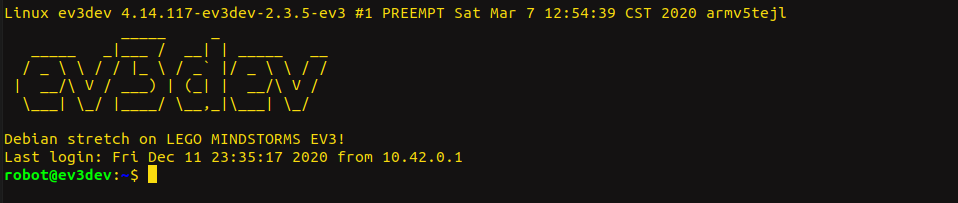
\includegraphics[width=0.8\textwidth]{img/ev3dev.png}
  \caption{Interfaz de la terminal de Ev3}
  \label{Diseño hardware del Ev3}
\end{figure}
Además crearon en \textit{Ev3dev} un entorno de software para programar el robot. Esto incluye soporte para muchos lenguajes de programación, entre ellos \textit{Python, Java o C++}. Para este proyecto he elegido utilizar el lenguaje \textit{Python}, ya que es uno de los lenguajes que comprende \textit{Kibotics} y estoy más familiarizado con él. 

\subsection{WebBrowser}

\subsubsection{Editor en el navegador web}

El editor de texto se encontrará entre la parrilla de ejercicios de \textit{Kibotics}. En este caso \textit{Kibotics} solo actua como plataforma que guarda los ejercicios que envió, y me proporciona la interfaz para poner el editor de texto que permita escribir su programa utilizando el lenguaje \textit{Python}. En el editor se importa la librería “\textit{Ev3dev2}”  que proporciona una API para interactuar con los sensores y actuadores del robot. Pero en este caso, \textit{Kibotics} no actúa en el envío, solo sirve la página para que podamos introducir el código.

\subsubsection{Envío del código al servidor Flask en el robot}

Utilizamos el editor \textit{ACE} para que el usuario escriba su código en la página Web, y cuando le de al botón \texttt{Enviar}, comienza el proceso de envío desarrollado en el script siguiente:
\\
\begin{lstlisting}[frame=single,breaklines=true, label=Función de envío del código al servidor, caption=Función de envío del código al servidor captionpos=b] <center><h3>En esta seccion podras enviar tu codigo  al LEGO Ev3.</h3></center>

<div class="text-center">
 <img class="text-center" src="{{ exercise.language }}/{{ exercise.exercise_id }}/img/ev3.png" width="300px" height="250px">
</div>

<div class="text-center">
  <img class="text-center" src="img/lego-mindstorms-education-ev3.jpg"
      width="300px" height="250px"
</div>

      <button type="button" id="send_mbot" class="btn btn-info" onclick="send_code_to_ev3()"><span
              class="glyphicon glyphicon-send"></span> Enviar
      </button>
</div>
\end{lstlisting}
Tras pulsar el botón \texttt{Enviar}, este código que hemos escrito en el editor se envía como un \textit{query parameter} de una petición POST. Desde el navegador se manda al servidor \textit{Flask} levantado en el robot. 
\\
\begin{lstlisting}[frame=single,breaklines=true, label=Función de envío del código al servidor, caption=Función de envío del código al servidor,  captionpos=b]
let responseOk;

  function send_code_to_ev3() {
      var editor = ace.edit("ace");
      let code = editor.getValue();
      console.log(code);
      const message = {
          method: "POST"
      };
      url = 'http://10.42.0.1:8001/run?python_code=' + JSON.stringify(code);
      fetch(url, message)
          .then(function(response) {
              if(response.ok){
                  responseOk = true
              }else{
                  responseOk = false
              }
              return response.text();
          })
          .then(function(data) {
               if(responseOk){
                  console.log("Ok")
              }else{
                  console.log("Send Fail")
              }

          })
          .catch(function(err) {
              console.error(err);
          });
  }
}
\end{lstlisting}
El servidor \texttt{Flask} hará la recepción del código que escribimos en el editor, y realizará determinadas acciones para que se pueda ejecutar en el \textit{LEGO EV3}


\subsection{Back-End}
El servidor que se ha creado, hace uso de \texttt{Flask} que es un entorno creado por \textit{Django} escrito en \textit{Python}, por lo que voy a programarlo en \textit{Python}. Esta creado para que reciba peticiones del navegador con el código que el usuario escribió en el editor



\begin{lstlisting}[frame=single,breaklines=true, label=Extracción del código en el servidor Flask, caption=Extracción del código en el servidor Flask,  captionpos=b]
import subprocess
import os
import signal
import time

from flask import Flask, make_response, request
app = Flask(__name__)   

exercice = None
@app.route('/run',methods=["POST"])
def run_program():
    global exercice
	my_json = request.data.decode('utf8').replace("'", '"')
    data = json.loads(my_json)
    code = json.dumps(data["code"])
    
    
#----------------------------------------------------------


if __name__ == "__main__":
    app.run(host='0.0.0.0', port=8001, debug=True)
\end{lstlisting}

\subsubsection{Creación del proceso que ejecuta la aplicación robótica}

Una vez ha recibido el código, el servidor ya sabe que el lenguaje en que viene es \textit{Python}, pero viene con algunos simbolos añadidos de HTML, por lo que se realizan dos \textit{replace} para dejarlo como estaba en origen.\newline
Una vez hecho este proceso, se procede a escribir un ejecutable con el código, para ello hay creado un archivo llamado \textit{ejercicio.py}.
Una vez creado el archivo se comprueba que no hay otro proceso ejecutándose, si es así se envía una señal \textit{kill} a dicho proceso.
Tras ejecutar el programa en un nuevo proceso, el robot realizará las instrucciones que el usuario programó en el editor del navegador web.
\\
\begin{lstlisting}[frame=single,breaklines=true, label=Creación del proceso con el programa para el robot, caption=Creación del proceso con el programa para el robot,  captionpos=b]
if exercice:
        try:
            os.killpg(os.getpgid(exercice.pid), signal.SIGKILL)
        except ProcessLookupError:
            pass

    time.sleep(2)
  
    code  = code[1:-1].split("\\n")
    print(code)
    fdOut = open("./ejercicio.py","w")
    for line in code:
            fdOut.write(line + "\n")
    
    exercice = subprocess.Popen(["python","ejercicio.py"],stdout=subprocess.PIPE,preexec_fn=os.setsid)
    
\end{lstlisting}

\subsubsection{Respuesta del Servidor}

Por último, se contesta al cliente con el código \textit{200 OK} 

\begin{lstlisting}[frame=single,breaklines=true, label=Respuesta del Servidor, caption=Creación del proceso con el programa para el robot,  captionpos=b]

headers = {'Content-Type': 'text/plain','Access-Control-Allow-Origin': '*'}
    return make_response('Ok', 200, headers)

\end{lstlisting}



\section{Validación experimental con Ejercicios}
\sectionmark{Validación Experimental}
En esta sección procedo a enviar dos ejercicios programados con las funciones de \textit{Kibotics} en el editor Web  para comprobar que lo que he contado anteriormente funciona. 
\subsection{Ejercicio Bump and go}
Para comprobar que todo lo anterior funciona hice tres ejercicios enviados desde un navegador web y ejecutados en el robot real. El primero, el \textit{BumpandGo} \footnote{\url{https://www.youtube.com/watch?v=5dD7O7Qku6I&ab_channel=DanielPulidoMillanes}} probando los el sensor de contacto.
\\
\begin{figure}[h!]
  \centering
    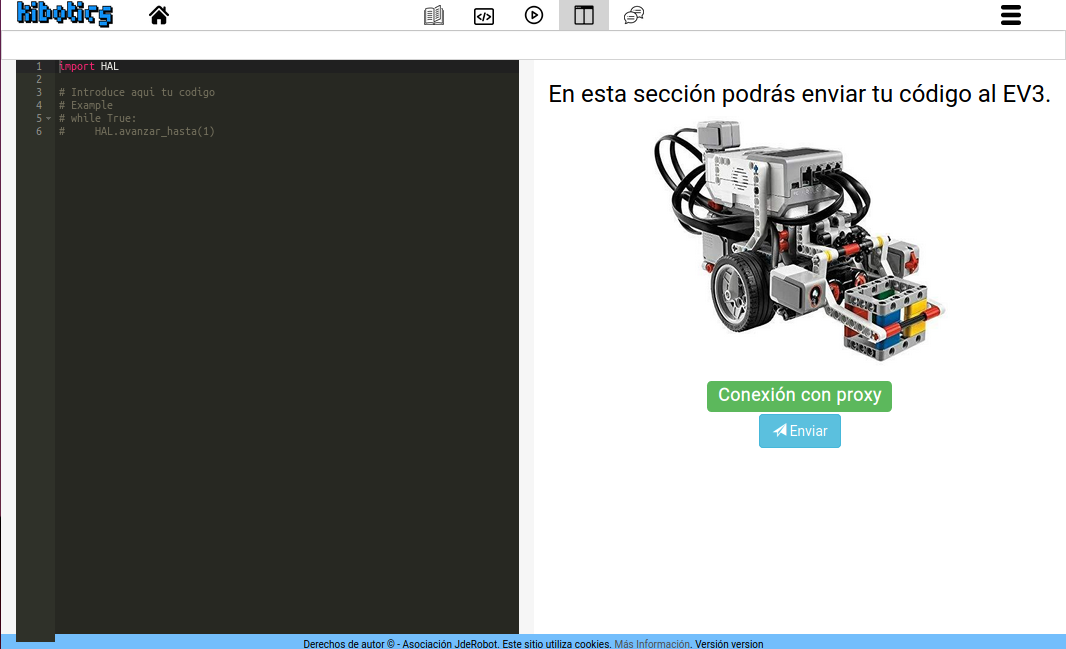
\includegraphics[width=0.8\textwidth]{img/editor_ev3.png}
  \caption{Editor Web para \textit{LEGO Ev3}}
  \label{Editor Web}
\end{figure}
\clearpage

En este apartado será donde insertemos el código que mandaremos al robot, para el caso del \textit{Bump and Go}:


\begin{lstlisting}[frame=single,breaklines=true, label=Bump and Go, caption=Bump and Go,  captionpos=b]

#!/usr/bin/env python3

import Ev3Wrapper
import time
Ev3 = Ev3Wrapper.Ev3Wrapper()

print("Bump and go!")

while True:
    if Ev3.IsTouching():
    	Eve.retroceder_hasta(10)
        Ev3.girar_derecha_hasta(120)
    else:
        Ev3.avanzar(30)
    # don't let this loop use 100% CPU
    sleep(0.01)

\end{lstlisting}



\subsection{Ejercicio Siguelineas}

El siguiente ejercicio que envié fue el \textit{Siguelineas}\footnote{\url{https://www.youtube.com/watch?v=iMn7UsaB2vo&ab_channel=DanielPulidoMillanes}} para también probar la función \textit{reflectedlightintensity} del sensor de color:
 
 \begin{lstlisting}[frame=single,breaklines=true, label=Siguelineas, caption=SigueLineas,  captionpos=b]

#!/usr/bin/env python3


#!/usr/bin/env python3

import Ev3Wrapper
import time
Ev3 = Ev3Wrapper.Ev3Wrapper()


print("Siguelineas!")

while True:
    while Ev3.getcolor(black)==1:
        Ev3.TurnDegrees(20,15)
    Ev3.TurnDegrees(-20,15)
    # don't let this loop use 100% CPU
    sleep(0.02)

\end{lstlisting}


